\section{Aufbau}
\label{sec:Aufbau}

Der Versuchsaufbau besteht aus einem Ultraschallechoskop und Ultraschallsonden verschiedener Frequenzen. 
Die Ultraschallsonden können sowohl für das Impuls-Echo-Verfahren als auch für das Durchschallungsverfahren genutzt werden.
Für die Datenaufnahme wird ein Rechner mit dem Programm A-Scan verwendet. In dem Versuch wird ein 
Acrylblock mit 11 Bohrungen, welcher in \autoref{fig:acryl} schematisch dargestellt ist, und ein Brustmodell 
mittels Ultraschall untersucht.

\begin{figure}
    \centering
    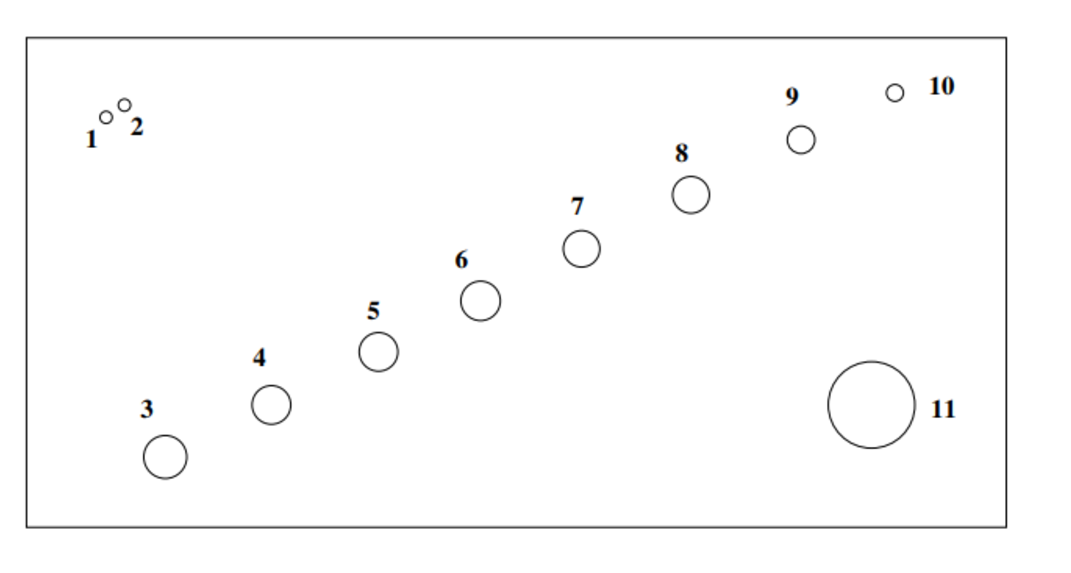
\includegraphics[height = 4cm]{block.pdf}
    \caption{Schematische Darstellung des verwendeten Acrylblocks \cite{apus1}.}
    \label{fig:acryl}
\end{figure}
